% ANNSIM 2027 — wersja polska (symulatory bramkowe a IQM Sirius). Wersja anonimowa.
% Szablon SCS z zestawu ANNSIM 2026 (scspaperproc, 5–12 stron); pliki klasy bez zmian.
\documentclass{scspaperproc}

\usepackage{latexsym}
\usepackage{graphicx}
\usepackage{mathptmx}
\usepackage{amsmath,amssymb}
\usepackage{booktabs}
\usepackage{placeins}
\usepackage[pdftex,colorlinks=true,urlcolor=blue,citecolor=black,anchorcolor=black,linkcolor=black,bookmarks=false]{hyperref}
\usepackage{hyphenat}
\sloppy
\usepackage[polish]{babel}
\hypersetup{pdftitle={ANNSIM 2027 Proceedings Paper}, pdfauthor={}, pdfsubject={ANNSIM 2027 Conference}}
\newcommand{\tofill}[1]{\textbf{[#1]}}
% the template title font (raw ptmb) has no Polish letters; same size and weight in T1 Times
\makeatletter\renewcommand\title[1]{\gdef\@title{\bfseries\fontsize{12}{14}\selectfont\MakeUppercase{#1}}}\makeatother

\begin{document}

\SCSpagesetup{Anonim}
\def\SCSconferencename{Annual Modeling and Simulation Conference}
\def\SCSconferenceacro{ANNSIM'27}
\def\SCSpublicationyear{2027}
\def\SCSconferenceeditors{\tofill{redaktorzy}}
\def\SCSconferencedates{May 17-21}
\def\SCSconferencevenue{Wroc{\l}aw University of Science and Technology, Wroc{\l}aw, Poland}

\author{}
\title{Na ile wiernie symulatory obwodów kwantowych przewidują sprzęt? Dziewięć
symulatorów i trzy scenariusze szumu wobec 16-kubitowego procesora o topologii
gwiazdy}

\maketitle

\section*{Streszczenie}
Symulatory niosą większość pracy nad algorytmami dla zaszumionych procesorów
kwantowych, ale rzadko sprawdza się, czy przewidują zachowanie urządzenia
w zadaniu, które symulacja zastępuje. Dziewięć darmowych symulatorów obwodów
dostaje kalibrację IQM Sirius, 16-kubitowego procesora o topologii gwiazdy,
i porównujemy je z urządzeniem na QAOA o stałych kątach, które wybiera ruchy
w iteracyjnym przeszukiwaniu lokalnym dla permutacyjnego problemu
przepływowego, w trzech scenariuszach szumu. Silniki, które obsługują dany
scenariusz, zgadzają się w granicach szumu próbkowania, więc wybór między nimi
jest kwestią kosztu, a z szumem wszystkie 16 kubitów obejmują tylko symulatory
trajektoriowe. Na całych przebiegach przeszukiwania symulatory z relaksacją
odtwarzają uszeregowania urządzenia w granicach jego własnego rozrzutu. Na
pojedynczych obwodach chybiają zmierzonych rozkładów mniej więcej dziesięć
razy bardziej, niż urządzenie różni się samo od siebie między dniami, co
wskazuje na relaksację kubitów w bezczynności, której nie modeluje żaden
scenariusz.

\textbf{Słowa kluczowe:} zaszumione procesory kwantowe, QAOA, permutacyjny problem przepływowy, benchmarking, topologia gwiazdy

\section{Wst\k{e}p}

Symulatory wykonują większość pracy przy urządzeniach kwantowych ery
NISQ~\cite{preskill2018}: czas procesora jest rzadki i drogi, więc algorytmy
projektuje się, stroi i często ocenia programowo, a urządzenie wykonuje tylko
końcowy eksperyment. Symulator jest przydatny o tyle, o ile przewiduje
zachowanie urządzenia, a jego wierność sprawdza się zwykle na syntetycznych
zestawach testowych~\cite{li2023qasmbench} albo mierzy się jego
szybkość~\cite{jamadagni2024bench}, a nie wynik zadania, które symulacja
zastępuje. Druga luka dotyczy samego sprzętu: procesory o topologii gwiazdy,
w których każdy kubit sprzęga się z centralnym rezonatorem przez osobną
operację MOVE, są nowe, a ekosystemy oprogramowania wspierają je
nierówno~\cite{gnatowski2026routing}.

Porównujemy dziewięć darmowych symulatorów obwodów z 16-kubitowym procesorem
o topologii gwiazdy, IQM Sirius, na zadaniu, którego wynik da się ocenić:
QAOA o stałych kątach~\cite{farhi2014qaoa} wybiera ruchy w iteracyjnym
przeszukiwaniu lokalnym dla permutacyjnego problemu
przepływowego~\cite{wojewodzki2026gcmm,wojewodzki2026aciids,wojewodzki2027icaisc}.
Wszystkie symulatory dostają te same dane kalibracyjne i trzy scenariusze
szumu o rosnącej szczegółowości. Oddzielamy wpływ silnika symulacji od wpływu
kompilatora, porównujemy wyniki symulowane z mierzonymi zarówno dla
pojedynczych obwodów, jak i dla końcowego harmonogramu, a każde porównanie
ograniczamy zgodnością sprzętu z samym sobą. Podajemy też koszt każdego
symulatora i miejsce, w którym przestaje działać. Symulatory zgadzają się ze
sobą i z urządzeniem co do wyniku przeszukiwania, ale nie co do tego, co
mierzy pojedynczy obwód, więc symulatorowi sprawdzonemu na końcowym
uszeregowaniu nie można ufać w przewidywaniu rozkładów wyników.

\section{Tło}

\paragraph{Zadanie.}
Zadaniem jest kwantowe przeszukiwanie sąsiedztwa w permutacyjnym problemie
przepływowym na instancjach Taillarda~\cite{taillard1993}. Iteracyjne
przeszukiwanie lokalne~\cite{lourenco2003} przechodzi od permutacji do
najlepszej permutacji w wykładniczym sąsiedztwie. Wybór tego ruchu to problem
kwadratowej optymalizacji binarnej bez ograniczeń (QUBO)~\cite{lucas2014ising}
nad kandydującymi zamianami: przekątna zawiera zmianę długości uszeregowania
każdej zamiany, a kara zabrania par konfliktowych. Permutacja 20 zadań wymaga
więcej zmiennych, niż mieści urządzenie, więc przeszukiwanie dzieli ją na
nakładające się okna i rozwiązuje jedno QUBO na okno algorytmem QAOA o stałych
kątach i głębokości $p$; ruch wybiera próbka o najniższej energii spośród 4096
shotów~\cite{wojewodzki2026aciids,wojewodzki2027icaisc}. Sąsiedztwa liniowe
(Adjacent, Fibonacci) dają okna od 1 do 16 zmiennych, a gęste (Dynasearch,
Motzkin) do 15.

\paragraph{Procesor o topologii gwiazdy.}
IQM Sirius sprzęga kubity z rezonatorem obliczeniowym. Oddziaływanie
dwukubitowe przenosi stan jednego kubitu do rezonatora, wykonuje bramkę CZ
z drugim kubitem i przenosi stan z powrotem, więc jedno oddziaływanie
$R_{ZZ}$ z QAOA kompiluje się do dwóch bramek CZ i około dwóch bramek MOVE.
Tabela~\ref{tab:calib} podaje kalibrację, która definiuje modele szumu;
skompilowany obwód ma o jeden kubit więcej niż okno, czyli rezonator.

\begin{table}[t]
\caption{Migawka kalibracji IQM Sirius z 23 października 2026 (16 działających
kubitów z 24; mediany po kubitach lub parach).}
\label{tab:calib}
\centering
\begin{tabular}{lr}
\toprule
Wielkość & Wartość \\
\midrule
Średnia wierność bramki PRX (jednokubitowej) & 0,9989 \\
Wierność CZ (kubit--rezonator) & 0,9833 \\
Wierność MOVE & 0,9903 \\
Błąd odczytu (średnia z $0\!\to\!1$ i $1\!\to\!0$) & 0,0175 \\
$T_1$ / $T_2$ kubitów & 30,0 / 10,9 $\mu$s \\
$T_1$ / $T_2$ rezonatora & 7,5 / 3,1 $\mu$s \\
Czasy bramek PRX / CZ / MOVE & 40 / 104 / 64 ns \\
\bottomrule
\end{tabular}
\end{table}

\paragraph{Kanały szumu.}
Kanał depolaryzujący o parametrze $\lambda$ zastępuje stan stanem maksymalnie
mieszanym z wagą $\lambda$; bramka o średniej wierności $F$ na układzie
o wymiarze $d$ daje $\lambda = d(1 - F)/(d - 1)$. Tłumienie amplitudy i fazy
modeluje relaksację energii ($T_1$) i dekoherencję fazy ($T_2$) w czasie
bramki, a macierz pomyłek dla każdego kubitu modeluje błędy odczytu. Symulator
może stosować kanały dokładnie na macierzy gęstości albo losować jedną gałąź
Krausa w każdym wykonaniu obwodu, co zamienia symulację z szumem w średnią po
trajektoriach~\cite{dalibard1992mcwf}. Druga droga kosztuje jedną symulację
wektora stanu na shot, ale zachowuje pamięć stanu czystego.

\section{Symulatory}

Tabela~\ref{tab:sims} zestawia programy; poniższe akapity opisują każdy z nich
i to, co oferuje dla symulacji z szumem przy 12--17 kubitach.

\paragraph{Qiskit Aer.}
Aer to warstwa symulacji Qiskita~\cite{javadi2024}. Oferuje gęsty wektor
stanu i macierz gęstości, stany iloczynowe macierzy oraz metody
stabilizatorowe, a szum przypina do pojedynczych instrukcji przez model
szumu. Z wektorem stanu Aer losuje jedną zaszumioną realizację obwodu na
shot, więc obsługuje pełne 17 kubitów skompilowanego obwodu dla Siriusa.
Adapter IQM dla Qiskita~\cite{iqmclient} kompiluje obwody do natywnych bramek
PRX, CZ i MOVE i buduje fałszywe backendy z architektury i profilu błędów,
z czego korzystamy, aby otrzymać model Siriusa z migawki kalibracji.

\paragraph{Cirq z qsim.}
Cirq~\cite{cirq} to framework Google do zapisu i kompilacji obwodów; qsim to
jego wydajny symulator wektora stanu w C++. Isakov i in.~\cite{isakov2021qsim}
opisują, jak qsim symuluje obwody z szumem jako trajektorie kwantowe,
losując wynik każdego kanału w czasie każdego wykonania, oraz jak opóźniony
iloczyn skalarny obniża koszt symulacji przy słabym szumie. Każde powtórzenie
wykonuje obwód od nowa, więc koszt rośnie z liczbą shotów. Adapter IQM dla
Cirqa, dziś część klienta IQM, odwzorowuje obwody na architektury IQM.

\paragraph{Qulacs.}
Qulacs~\cite{suzuki2021qulacs} to symulator w C++ z interfejsem w Pythonie,
zbudowany z myślą o szybkości dla małych i średnich obwodów. Modeluje szum
jako bramki probabilistyczne (depolaryzację jedno- i dwukubitową, dekoherencję
fazy i przerzut bitu) oraz jako ogólne odwzorowania całkowicie dodatnie
zadane operatorami Krausa, co obejmuje tłumienie amplitudy; przechowuje też
macierze gęstości. Docieramy do niego przez TKET~\cite{sivarajah2020tket},
którego rozszerzenie IQM daje trzeci kompilator dla topologii gwiazdy.

\paragraph{MQT DDSIM.}
DDSIM reprezentuje stany i operacje jako diagramy decyzyjne, które kompresują
redundancję wielu obwodów~\cite{zulehner2019ddsim}. Jego tryb z szumem
symuluje dekoherencję i błędy bramek stochastycznie albo deterministycznie, na
diagramach decyzyjnych dla macierzy gęstości~\cite{grurl2020noise}.
Udokumentowany interfejs stosuje tłumienie amplitudy, depolaryzację i przerzut
fazy z jednym globalnym prawdopodobieństwem, więc skalibrowane wartości dla
poszczególnych bramek mogą wejść tylko jako średnia.

\paragraph{Qibo.}
Qibo~\cite{efthymiou2022qibo} to framework do symulacji z akceleracją
sprzętową na CPU i GPU. W pierwotnym opisie obwód z kanałami szumu przełącza
symulację na macierze gęstości, których pamięć rośnie jak $4^n$; z szumem
obsługuje więc mniejsze okna naszego zadania.

\paragraph{CUDA-Q.}
CUDA-Q~\cite{kim2023cudaq} to platforma NVIDIA dla programów
hybrydowych kwantowo-klasycznych. Jej dokumentacja stosuje modele szumu na
backendzie macierzy gęstości na CPU; na komputerze bez GPU NVIDIA ogranicza
to przebiegi z szumem do małych okien.

\paragraph{PennyLane.}
PennyLane~\cite{bergholm2018pennylane} skupia się na różniczkowalnych
programach hybrydowych. Jego urządzenie dla stanów mieszanych symuluje kanały
szumu na macierzach gęstości i jest zalecane dla małych układów; modele szumu
zapisane dla Qiskita można zaimportować, co ułatwia porównanie jeden do
jednego.

\paragraph{Amazon Braket.}
SDK Braket~\cite{braket} zawiera lokalne symulatory wektora stanu i macierzy
gęstości; lokalny symulator macierzy gęstości obsługuje obwody z szumem
o około dwunastu kubitach, a większe działają w płatnej usłudze chmurowej,
z której nie korzystamy.

\paragraph{QuTiP.}
QuTiP~\cite{johansson2013qutip,lambert2024qutip5} symuluje otwarte układy
kwantowe przez równania master. Jego pakiet obwodów symuluje obwody na poziomie
impulsów sterujących z szumem~\cite{li2022qutipqip}, czyli opisem poniżej
poziomu bramek, którego używają pozostałe programy; stosujemy go na jednym
małym oknie jako odniesienie dla tego poziomu szczegółowości.

\paragraph{Stim i powód jego wykluczenia.}
Stim~\cite{gidney2021stim} bardzo szybko symuluje obwody stabilizatorowe i jest
standardowym narzędziem w badaniach korekcji błędów. Obwody QAOA zawierają
dowolne obroty i nie są obwodami Clifforda, więc Stim nie wykona naszego
zadania.

\paragraph{Pokrewne porównania.}
Testy pakietów symulacyjnych mierzą szybkość na wektorze stanu bez
szumu~\cite{jamadagni2024bench} albo dostarczają obwodów
testowych~\cite{li2023qasmbench}. Georgopoulos i in.~\cite{georgopoulos2021noise}
zbudowali model szumu z parametrów urządzenia i porównali go z przebiegami na
sprzęcie. Dokładamy trzy rzeczy: wiele symulatorów zasilanych tą samą
kalibracją, procesor o topologii gwiazdy i porównanie na wyniku zadania
optymalizacyjnego.

\begin{table}[t]
\caption{Tabela podaje metodę z szumem każdego symulatora według jego
dokumentacji. Zmierzone granice podaje tabela~\ref{tab:t6}.}
\label{tab:sims}
\centering
\small
\begin{tabular}{llll}
\toprule
Symulator & Metoda z szumem & Kompilator IQM & Licencja \\
\midrule
Qiskit Aer & trajektorie, macierz gęstości & qiskit-iqm & Apache-2.0 \\
Cirq + qsim & trajektorie & klient IQM (Cirq) & Apache-2.0 \\
Qulacs & bramki probab., Kraus & przez TKET & MIT \\
MQT DDSIM & diagramy decyzyjne & --- & MIT \\
Qibo & macierz gęstości & --- & Apache-2.0 \\
CUDA-Q (CPU) & macierz gęstości & --- & Apache-2.0 \\
PennyLane & macierz gęstości & --- & Apache-2.0 \\
Braket (lokalnie) & macierz gęstości & --- & Apache-2.0 \\
QuTiP & równania master (impulsy) & --- & BSD-3 \\
Stim & tylko stabilizatory & --- & Apache-2.0 \\
\bottomrule
\end{tabular}
\end{table}

\section{Metodyka}

\paragraph{Scenariusze szumu.}
Wszystkie symulatory korzystają z tej samej migawki kalibracji i trzech
scenariuszy. W S1 obwód działa bez szumu. W S2 każda bramka ma kanał
depolaryzujący dopasowany do zmierzonej wierności, a każdy kubit macierz
pomyłek odczytu. S3 dodaje tłumienie amplitudy i fazy w czasie każdej bramki.
Na Siriusie sama relaksacja przekracza zmierzony błąd większości bramek
(mediana błędu CZ: zmierzona 0,0167 wobec 0,0205 wynikającej z $T_1$ i $T_2$),
więc S3 ogranicza szum od góry. Żaden scenariusz nie modeluje bezczynnych
kubitów; każdy symulator stosuje szum tylko w czasie bramek. Symulatory szumu
DDSIM zawodzą już na obwodach bez szumu, więc DDSIM liczy tylko S1.

\paragraph{Dwa tory.}
W torze A każdy symulator wykonuje ten sam skompilowany obwód, wyeksportowany
jako lista bramek natywnych z bramką MOVE zapisaną jako zamiana między kubitem
a rezonatorem, więc każda różnica pochodzi z silnika i jego kanałów. W torze B
ten sam obwód logiczny przechodzi przez dwa kompilatory (adaptery IQM dla
Qiskita i Cirqa) i wykonuje się w jednym silniku, więc różnice pochodzą
z kompilacji.

\paragraph{Odniesienie sprzętowe.}
Tabela~\ref{tab:hw} wymienia dane z urządzeń. Porównania na poziomie
przebiegów korzystają z iteracyjnego przeszukiwania lokalnego na Siriusie przy
$p = 1$ z wcześniejszej kampanii~\cite{wojewodzki2026aciids}. Porównania na
poziomie obwodów wymagają histogramów pojedynczych okien. Bieg H3 wykonuje 84
obwody pierwszego ruchu instancji 0 klasy tai20 przy $p = 1, 2$ w dwa dni
(6 i 7 listopada 2026), po 4096 shotów, a symulatory odtwarzają skompilowane
obwody z kalibracją z tego samego dnia.

\paragraph{Miary.}
Dla pojedynczych obwodów porównujemy średnią energię QUBO próbek,
znormalizowaną tak, że 0 to optimum, a 1 najgorsze przypisanie, oraz to, czy
ruch optymalny w ogóle pojawia się w próbce. Podajemy też odległość
całkowitej zmienności, ale przy 4096 shotach i do $2^{15}$ możliwych wynikach
mierzy ona głównie szum próbkowania. Podłogą sprzętową jest różnica między
dwoma dniami biegu H3. Dla całych przebiegów porównujemy względne odchylenie
długości uszeregowania od dolnego ograniczenia Taillarda po tej samej liczbie
ruchów, jaką wykonało urządzenie, testem Wilcoxona dla par z poprawką Holma
i przedziałem bootstrap po instancjach; podłogę dają powtórzone przebiegi
urządzenia. Koszt to czas na obwód i szczytowa pamięć.

\section{Plan eksperymentów}

Badanie przebiega w trzech etapach. Najpierw każdy symulator jest instalowany
i sprawdzany na jednym oknie. Następnie wszystkie symulatory, które mogą
wykonać dany scenariusz, liczą okna instancji 0--3 klas Taillarda
z $n = 20$ zadaniami: 161 okien z ruchem poprawiającym, z których 71 ma co
najwyżej 11 zmiennych i mieści się w symulatorach macierzy gęstości. Na końcu
qsim i Qulacs, czyli dwa symulatory, które najtaniej obejmują z szumem
wszystkie 16 kubitów, odtwarzają 153 przebiegi urządzenia dla $n = 50$ do
$500$ w scenariuszu S2.

\begin{table}[t]
\caption{Dane sprzętowe użyte jako odniesienie, wszystkie zebrane w 2026~r. Przebiegi H2
podajemy dla kompletności; w tej pracy ich nie używamy.}
\label{tab:hw}
\centering
\small
\setlength{\tabcolsep}{4pt}
\begin{tabular}{llll}
\toprule
Urządzenie & Eksperyment & Zakres & Data \\
\midrule
IQM Sirius & ILS, $p = 1$, 10 s & 12 klas ($n = 20$--$500$), inst.\ 0--3; 225 przebiegów & 7--14.10 \\
IQM Sirius & ILS, $p = 2, 3$ (H2) & $n = 20$, inst.\ 0--3; 96 przebiegów & XI \\
IQM Sirius & histogramy (H3), dwa dni & tai20, inst.\ 0, $p = 1, 2$ & 6--7.11 \\
IBM Heron (ibm\_fez) & jeden ruch na przebieg, $p = 1$ & tai20\_5, inst.\ 0--9 & VIII \\
IQM Garnet, Emerald & jeden ruch na przebieg, $p = 1$ & tai20\_5, inst.\ 0 & IX--X \\
\bottomrule
\end{tabular}
\end{table}

\section{Wyniki}

Każdy symulator, który obsługuje dany scenariusz, odtwarza te same rozkłady.
Metody dokładne zgadzają się do precyzji maszynowej, a próbkujące mieszczą się
w progu szumu próbkowania we wszystkich oknach poza kilkoma procentami, których
należy się spodziewać przez przypadek. Wyjątkami są przypadki, w których
program zawodzi: symulatory szumu DDSIM zwracają złe rozkłady nawet bez szumu
i wywracają się na większych oknach, metoda trajektorii Aer kończy się
błędem, gdy S3 dodaje relaksację, a symulator szumu Qulacs nigdy nie stosuje
tłumienia amplitudy. Wybór silnika nie zmienia więc przewidywania, tylko jego
koszt.

Ten koszt pokazują rysunek~\ref{fig:cost} i tabela~\ref{tab:t6}. Symulatory
macierzy gęstości kończą się na dziewięciu do trzynastu kubitach przy limicie
300\,s na obwód, a metody trajektorii qsim i Qulacs obejmują z szumem wszystkie
16 kubitów Siriusa. Qulacs jest najszybszym programem przy każdym rozmiarze.
Jego jawna pętla po shotach potrzebuje tylko pamięci stanu czystego,
a wbudowany symulator szumu jest nieco szybszy, ale zajmuje gigabajty i liczy
S3 źle. Trajektorie Qibo są poprawne, ale o jeden do dwóch rzędów wielkości
wolniejsze.

Kompilator ma większe znaczenie niż silnik. Adapter IQM dla Cirqa kompiluje te
same obwody z tą samą liczbą bramek CZ co adapter dla Qiskita, ale z 30--60\,\%
większą liczbą bramek MOVE (tabela~\ref{tab:compilers}), a przy $p = 2$
dodatkowy szum sprawia, że próbka o najniższej energii rzadziej jest ruchem
optymalnym.

Na całych przebiegach ILS z budżetem ruchów urządzenia scenariusza
z relaksacją nie da się odróżnić od Siriusa dla żadnego z dwóch symulatorów
(rysunek~\ref{fig:prd}, tabela~\ref{tab:t5}). Średnie odchylenie od dolnego
ograniczenia różni się o mniej niż pół punktu procentowego, czyli dużo mniej
niż dwa przebiegi samego urządzenia. Bez relaksacji qsim daje istotnie gorsze
uszeregowania niż urządzenie, a Qulacs wskazuje ten sam kierunek, choć bez
istotności. Na większych instancjach ($n = 50$ do $500$, 153 przebiegi urządzenia)
scenariusz S2 obu symulatorów daje uszeregowania o około 0,4 punktu procentowego gorsze niż
urządzenie. Różnica jest mała, ale systematyczna, pochodzi z sąsiedztw gęstych i maleje ze
wzrostem $n$. Urządzenie wykonało w tych przebiegach jeden ruch, więc na największych
instancjach długość uszeregowania niewiele odbiega od początkowej, a zgodność mówi więcej
o budżecie niż o symulatorach.

Na pojedynczych obwodach tej zgodności nie ma. Urządzenie dobrze odtwarza samo
siebie, bo średnia energia obwodu zmienia się między dniami o mniej niż
0,01, ale każdy symulator w każdym scenariuszu chybia o mniej więcej dziesięć
razy więcej (rysunek~\ref{fig:h3}, tabela~\ref{tab:h3}). Przy $p = 1$
urządzenie wypada lepiej niż symulacja bez szumu: ruch optymalny pojawia się
w 79 z 84 histogramów, wobec 46 w S1, a jego próbki zawierają mniej jedynek.
Ruch optymalny ustawia na jeden niewiele zmiennych, więc dryf kubitów w stronę
stanu podstawowego mu sprzyja, a taki skutek miałaby relaksacja kubitów
w bezczynności. Przy $p = 2$ scenariusze S2 i S3 trafiają średnią energię
wszystkich obwodów, ale spłaszczają różnice między obwodami, które widać na
urządzeniu.

\begin{table}[t]
\caption{Tabela podaje medianę liczby bramek CZ i MOVE na okno po kompilacji
($p = 1$, 161 okien).}
\label{tab:compilers}
\centering
\small
\begin{tabular}{lcc}
\toprule
Sąsiedztwo & qiskit-iqm (CZ / MOVE) & IQM Cirq (CZ / MOVE) \\
\midrule
Adjacent & 72 / 72 & 72 / 92 \\
Fibonacci & 16 / 16 & 16 / 20 \\
Dynasearch & 164 / 178 & 164 / 286 \\
Motzkin & 134 / 144 & 134 / 214 \\
\bottomrule
\end{tabular}
\end{table}

\begin{figure}[t]
\centering
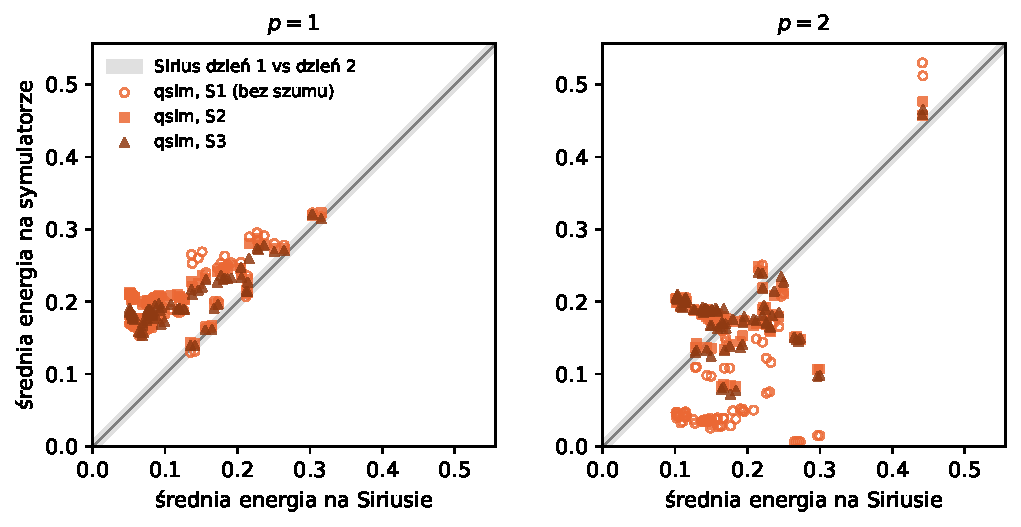
\includegraphics[width=0.8\textwidth]{figures/h3_energy_pl.pdf}
\caption{Każdy punkt to jeden obwód H3 z jednego dnia. Szary pas pokazuje
średnią różnicę między dwoma dniami na Siriusie.}
\label{fig:h3}
\end{figure}

\begin{table}[t]
\caption{Tabela porównuje średnią znormalizowaną energię QUBO (0 to optimum) 84 obwodów H3 z dwóch dni. $|\Delta E|$ to średnia różnica od Siriusa na obwód, a sam Sirius różni się między dniami o 0{,}006--0{,}008.}
\label{tab:h3}
\centering
\small
\begin{tabular}{clccccc}
\toprule
$p$ & Źródło & $E$ qsim & $E$ Qulacs & $|\Delta E|$ & optimum w próbce & jedynki \\
\midrule
1 & Sirius & \multicolumn{2}{c}{0{,}118} & 0{,}006 & 79/84 & 3{,}20 \\
 & S1 (bez szumu) & 0{,}199 & 0{,}200 & 0{,}081 & 46/84 & 4{,}69 \\
 & S2 & 0{,}214 & 0{,}214 & 0{,}096 & 43/84 & 4{,}95 \\
 & S3 & 0{,}199 & 0{,}198 & 0{,}081 & 47/84 & 4{,}75 \\
\midrule
2 & Sirius & \multicolumn{2}{c}{0{,}177} & 0{,}008 & 71/84 & 4{,}25 \\
 & S1 (bez szumu) & 0{,}082 & 0{,}082 & 0{,}100 & 82/84 & 2{,}26 \\
 & S2 & 0{,}182 & 0{,}182 & 0{,}054 & 65/84 & 4{,}55 \\
 & S3 & 0{,}182 & 0{,}183 & 0{,}055 & 70/84 & 4{,}57 \\
\bottomrule
\end{tabular}
\end{table}


\begin{figure}[t]
\centering
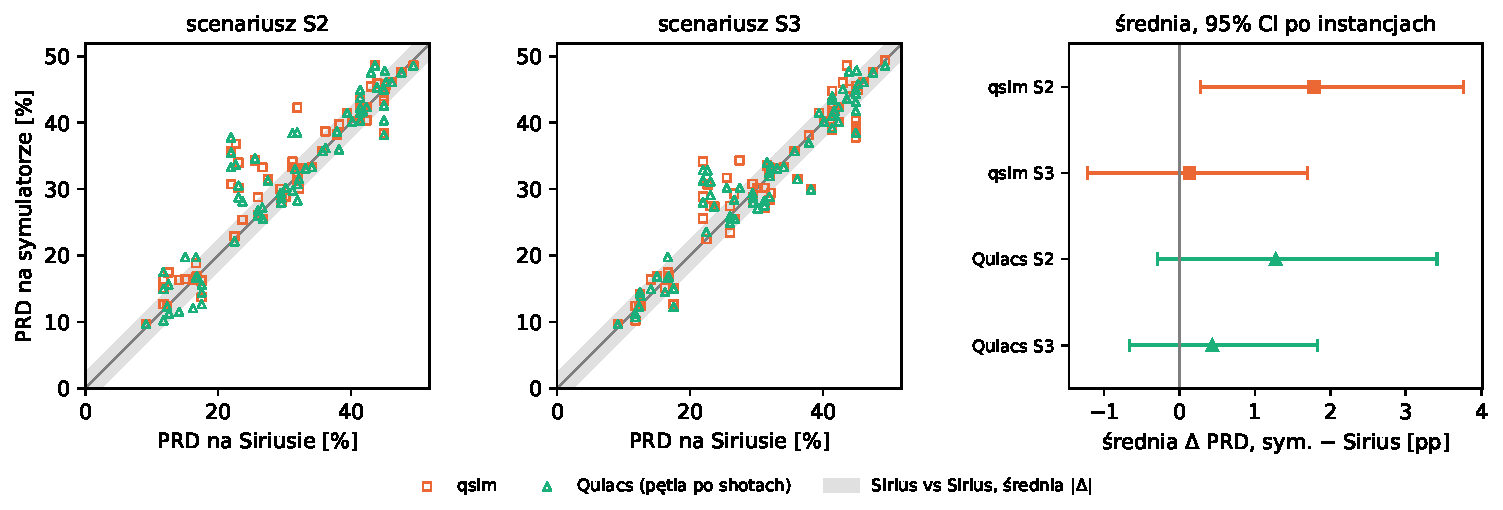
\includegraphics[width=\textwidth]{figures/t5_prd_pl.pdf}
\caption{Każdy punkt to jeden bieg ILS na symulatorze i na Siriusie (tai20,
$p = 1$). Szary pas pokazuje średnią różnicę dwóch biegów Siriusa, a prawy panel
pokazuje średnią różnicę z 95\,\% CI.}
\label{fig:prd}
\end{figure}

% generated by src/simulation/t5_stats.py
\begin{table}[t]
\caption{Tabela porównuje średni PRD 72 sparowanych biegów ILS na symulatorze i na Siriusie. $\Delta$ to różnica symulator minus Sirius w pp, CI to 95\,\% przedział po instancjach, a $p$ pochodzi z testu Wilcoxona z poprawką Holma. Sirius osiąga średni PRD 30,70.}
\label{tab:t5}
\centering
\small
\setlength{\tabcolsep}{4pt}
\begin{tabular}{llccccc}
\toprule
Symulator & Sc. & PRD & $\Delta$ & 95\,\% CI & lepszy / remis / gorszy & $p$ \\
\midrule
qsim & S2 & 32,48 & $+1{,}78$ & $[+0{,}28; +3{,}77]$ & 18 / 15 / 39 & 0,00098 \\
qsim & S3 & 30,83 & $+0{,}13$ & $[-1{,}21; +1{,}70]$ & 26 / 17 / 29 & 0,94 \\
Qulacs (pętla po shotach) & S2 & 31,98 & $+1{,}28$ & $[-0{,}29; +3{,}41]$ & 23 / 18 / 31 & 0,12 \\
Qulacs (pętla po shotach) & S3 & 31,13 & $+0{,}43$ & $[-0{,}66; +1{,}83]$ & 28 / 16 / 28 & 0,94 \\
\bottomrule
\end{tabular}
\end{table}


\begin{figure}[t]
\centering
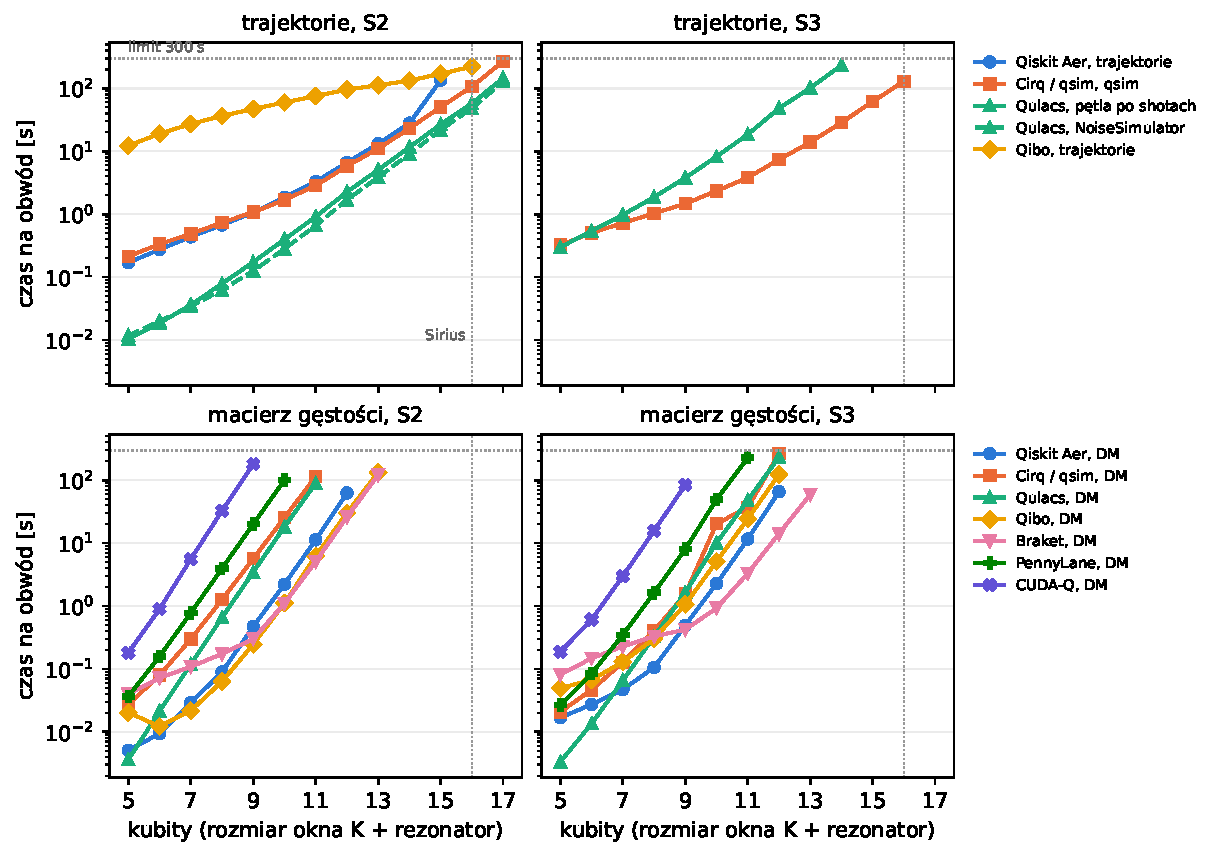
\includegraphics[width=\textwidth]{figures/t6_cost_pl.pdf}
\caption{Wykres pokazuje czas na obwód w funkcji liczby kubitów ($p = 1$,
jeden wątek). Linie kropkowane oznaczają limit 300\,s i 16 kubitów Siriusa.}
\label{fig:cost}
\end{figure}

% generated by src/simulation/t6_plot.py
\begin{table}[t]
\caption{Tabela podaje największe okno $K$, które mieści się w 300\,s na obwód, czas przy $K = 11$ w S2 i szczytową pamięć ($p = 1$, jeden wątek). Krzyżyk oznacza błąd biblioteki lub zły rozkład, a --- oznacza scenariusz bez obsługi.}
\label{tab:t6}
\centering
\small
\begin{tabular}{llccccr}
\toprule
Program & Metoda & \multicolumn{3}{c}{maks.\ $K$} & $t$ [s], S2, $K = 11$ & RSS S2 [MB] \\
 & & S1 & S2 & S3 & & \\
\midrule
Qiskit Aer & trajektorie & 16 & 14 & 4$^\dagger$ & 6,62 & 113 \\
Cirq / qsim & qsim & 16 & 16 & 15 & 5,8 & 239 \\
Qulacs & pętla po shotach & 16 & 16 & 13 & 2,26 & 106 \\
Qulacs & NoiseSimulator & 16 & 16 & 13$^\dagger$ & 1,69 & 9092 \\
Qibo & trajektorie & 16 & 15 & --- & 95,6 & 284 \\
Qiskit Aer & DM & 12 & 11 & 11 & 62,9 & 366 \\
Cirq / qsim & DM & 12 & 10 & 11 & --- & 719 \\
Qulacs & DM & 12 & 10 & 11 & --- & 277 \\
Qibo & DM & 12 & 12 & 11 & 30,1 & 4630 \\
Braket & DM & 16 & 12 & 12 & 26 & 6064 \\
PennyLane & DM & 16 & 9 & 10 & --- & 310 \\
CUDA-Q & DM & 16 & 8 & 8 & --- & 225 \\
\bottomrule
\end{tabular}
\end{table}


\FloatBarrier
\section{Dyskusja i wnioski}

W badaniu takim jak to każdy symulator trajektoriowy przewiduje wynik
optymalizacji tak dobrze jak drugi przebieg na urządzeniu, pod warunkiem że
jego model szumu zawiera relaksację, a Qulacs robi to najtaniej. Zgodność
w dużej mierze zawdzięczamy odczytowi w przeszukiwaniu, który zachowuje
najlepszą z 4096 próbek i nie zależy od kształtu rozkładu. Te same symulatory
zawodzą, gdy pytanie dotyczy samego rozkładu, na przykład prawdopodobieństwa
ruchu optymalnego albo wpływu głębokości, i tam urządzenie zachowuje się
w sposób, którego nie przewiduje żaden scenariusz. Najbardziej
prawdopodobnym brakującym składnikiem jest szum kubitów w bezczynności:
w procesorze gwiazdowym każda bramka dwukubitowa przechodzi przez rezonator,
więc większość kubitów czeka przez większość obwodu.

Te wnioski mają granice. Symulacje przebiegów korzystają z jednej migawki
kalibracji, wszystkie modele szumu traktują rezonator jak kubit, dane na
poziomie obwodów obejmują jedną klasę instancji przy dwóch głębokościach,
a powyżej $n = 20$ porównanie przebiegów obejmuje tylko scenariusz S2 i przebiegi
z jednym ruchem.
Kolejnym krokiem jest scenariusz z szumem bezczynności zbudowany
z harmonogramu skompilowanych obwodów i sprawdzony na tych samych
histogramach.

\bibliographystyle{scsproc}
\bibliography{references}
\end{document}
